% Preamble
\documentclass[9pt,oneside,headheight=10mm]{book}


% Packages
\usepackage{amsmath}    % American Math Socitey distributed package
\usepackage{amsfonts}	% Ams Fonts
\usepackage[a4paper, total={7in, 9.5in}]{geometry}   % Page size and margin
\usepackage{ulem}   % Package for underlines
%\usepackage{LobsterTwo} % Font package LobsterTwo
%\usepackage[math]{kurier}   % Font package kurier (with math support)
\usepackage[T1]{fontenc}    % Package for font encoding (You are able to select fonts)
\usepackage{graphicx}   % Package for including images
\usepackage[x11names]{xcolor}   % Adds more color and enables customize colors
\usepackage{color}  % Font color
\usepackage{afterpage}   % Set multiple pages in one line
\usepackage{utfsym} % More symbols
\usepackage{titlesec}   % Program title format for environments
\usepackage{sectsty}    % Section title color
\usepackage{fancyhdr}   % Make headers and footers
\usepackage{tipa} 	% ipa charts
\usepackage{tikz}	% Graphing tool
\usepackage{pgffor}	% For loops
\usepackage{hyperref}
\usepackage{multicol}
\usepackage{mathtools}

\usepackage{xeCJK}

% tikz drawing packages
\usetikzlibrary{arrows.meta}
\usetikzlibrary{patterns}
\usetikzlibrary {datavisualization.formats.functions}
\usetikzlibrary{bending}
\usetikzlibrary{shapes}



% Other Settings
\setlength{\fboxrule}{1.2pt}    % Setting width of fbox
\graphicspath{ {./images/} }    % Setting defulat image path
\definecolor{umYellow}{HTML}{FFCB05}    % Defining color - umYellow
\definecolor{umBlue}{HTML}{00274C}      % Defining color - umBlue


% Set Environment Appearance & New enviornments
\allsectionsfont{\color{umBlue}}
\newtheorem{theorem}{\color{umBlue}Theorem}[section]
\newtheorem{ex}{\color{umBlue}Example}[section]
\newtheorem{defn}{\color{umBlue}Definition}[section]
\newtheorem{coro}{\color{umBlue}Corollary}[theorem]
\newtheorem{lemma}{\color{umBlue}Lemma}[theorem]

\setlength{\parskip}{0.1cm} % Distance Between Paragraphs
\setlength{\parindent}{22pt}    % Indent first line of parargraph



% New Commands
\newcommand{\bm}[1]{\begin{bmatrix}#1\end{bmatrix}}
\newcommand{\cb}[1]{\left(#1\right)}
\newcommand{\bra}[1]{\left<#1\right|}
\newcommand{\ket}[1]{\left|#1\right>}
\newcommand{\sqb}[1]{\left[#1\right]}
\newcommand{\pp}{\partial}
\newcommand{\tx}[1]{\text{#1}}
\newcommand{\vs}[1]{\vspace{#1}}
\newcommand{\solution}{\color{umBlue}$~~~~$\textit{solution.}\color{black}\\}
\newcommand{\proof}{\color{umBlue}$~~~~$\textit{proof.}\color{black}\\}
\newcommand{\qed}{\hfill$\blacksquare$}
\newcommand{\cut}{\backslash}
\newcommand{\dbar}{\text{\dj}}
\newcommand{\blue}{\color{blue}}
\newcommand{\black}{\color{black}}
\newcommand{\blueit}[1]{\textit{\blue #1\black}}
\newcommand{\bluebf}[1]{\textbf{\blue #1\black}}


% Document
\begin{document}
    \parindent 0ex
    % Configure Header and Footer
    \pagestyle{fancy}
    \fancyhead{} % clear all header fields
    \fancyhead[CO,CE]{\leftmark}    % Get section name displayed in header

    \pagecolor{umBlue}
    \begin{titlepage}
        \color{umYellow}
        \begin{center}
            
\includegraphics[width=4cm]{umichlogo}\\
            \vspace*{1.5cm}
            \fbox{\parbox{\linewidth}{\begin{center}
                \huge 
           
            \textbf{Reading Notes for Physics 535\\
           	General Relativity}\\   % Title
              
                \normalfont
                \vspace*{6pt}
                \large Professor: Leopoldo A. Pando Zayas\\ % Author/Lecturer
                \vspace*{4pt}
                \rule{14cm}{0.6pt}\\
                \vspace*{4pt}
                Notes provided by: Chi Han (University of Michigan) \\    % Self
                \today
                \end{center}
            }}

            \vspace*{1.5cm}
           
        \end{center}
    \end{titlepage}

    \pagecolor{white}   % Set page color for all following pages
    \afterpage
    
    \tableofcontents
    
    
    
    
    
    
    
    
	\newpage
	\chapter{$k$-Calculus}
	\section{Galilean Transformation}
	In Newtonian mechanics, we apply Galilean transformations when changing perspectives between (inertial) frames. Suppose a point $P$ in frame $S'$ is measured to have spacetime coordinate $P_{S'}(x',y',z', t')$, with \bluebf{Galilean transformation}, its spacetime coordinate in $S$ is given by:
	\begin{align*}
	P_S (x'+vt,y',z', t')
	\end{align*}
	
	\section{Principles of Special Relativity}
	We start with a theory that underpins the Newtonian theory. 
	
	\begin{center}
	
	
	\fbox{\parbox{14cm}{\bluebf{restricted principle of special relativity}
	
	\vspace*{0.3cm}	
	All inertial observers are equivalent as far as the dynamical experiments are concerned.
	}}
	
	\end{center}
	This states that observers should observe the same result for identical dynamical experiments that are performed in  inertial frames. However, Einstein realized that there are no \textit{purely dynamical} experiments, and therefore modified the statement and obtained the first postulate of special relativity.
	\begin{center}
	
	
	\fbox{\parbox{14cm}{\bluebf{Postulate I. Principle of Special Relativity}
	
	\vspace*{0.3cm}	
	All inertial observers are equivalent.
	}}
	
	\end{center}
	
	\section{The Constancy of Velocity of Light}
	To describe events (points in spacetime) with $k$-calculus, we use ``radar methods'' to measure time and distance, that is, sending light signals to the event and receive the signal reflected from it. By setting the speed of light equals 1 with natural units, we can define the distance of an object by half of the time difference between emission and reception. The reason to use light is the second postulate, which resulted from observation on binary stars.
	\begin{center}
	
	
	\fbox{\parbox{14cm}{\bluebf{Postulate I. Constancy of Velocity of Light}
	
	\vspace*{0.3cm}	
	The velocity of light $c$ is the same in all inertial systems.
	}}
	
	\end{center}
	Physically, the velocity of light takes a numerical value of $c = 2.9979\times 10^8$m/s. However, in discussions about relativity, we usually adopt natural units, in which $c:=1$.
	
	\section{Lorentz Transformation}
	From the two postulates, we are able to derive the transformation, equivalent to Galilean's, but in a relativistic configuration.
	
	Suppose frame $S'$ is moving (away) at a speed $v$ with respect to frame $S$ in $x$-direction. Given the measurements $P(x,y,z,t)$ in frame $S$, the measurement by an observer in frame $S'$ is given by:
	\begin{align*}
	P'\cb{\frac{t-vx}{\sqrt{1-v^2}}, \frac{x-vt}{\sqrt{1-v^2}}, y, z}
	\end{align*}
	We noticed that:
	\begin{align*}
	\lim_{v\to 0}P' = P
	\end{align*}
	\section{The Four-Dimensional World View}
	In Lorentz transformation, we see $x$ dependence in $t$, this is a major difference from Galilean point of view, in which the absolute time frame is invariant. It is also useful to notice the symmetry in space and time, and the mixing of space and time. Quoting Minkowski, ``Henceforth space byitself, and time by itself are doomed to fade away into mere shadows, and only a kind of union of the two will preserve an independent reality'', we try to discover a quantity that remains invariant under Lorentz Transformations like $\Delta t$ and $\Delta r$ under Galilean Transformations.
	
	We define the metric in Minkowski space-time $\cb{\text{the space of } (t,x,y,z)\in\mathbb{R}^4}$ to be
	\begin{align*}
	\Delta s^2 = (t_1-t_2)^2 - (x_1-x_2)^2 - (y_1-y_2)^2 - (z_1-z_2)^2
	\end{align*}
	It is the squared interval between events $(t_1, x_1, y_1, z_1)$ and $(t_2, x_2, y_2, z_2)$. Infinitesimally, we have:
	\begin{align*}
	ds^2 = dt^2 - dx^2 - dy^2-dz^2
	\end{align*}
	This quantity ($\Delta s^2$, or $ds^2$) is invariant under Lorentz Transformation.\\
	Note, the Lorentz Transformation defined in the previous section is only the valid when the two frames are oriented in the standard way - the relative velocity between the two are in $x$-direction. When dealing with a more general orientation case, one can always apply rotation to turn the configuration in to a standard one, as long as the relative velocity $v$ is a fixed vector without acceleration.
	
	\section{The $k$-factor}
	We can finally introduce $k$-calculus in the study of special relativity. For simplicity, let's start from 2-dimension spacetime (t,x).
	\begin{center}
	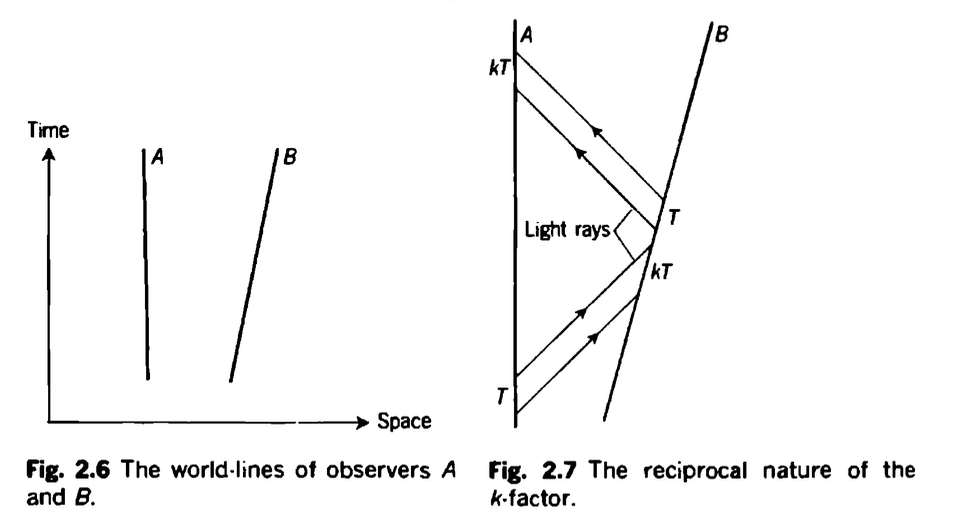
\includegraphics[width=12cm]{Chap1/1-1}\\
	Figure 1-1: World lines of observer $A$ in $S$ and $B$ in $S'$, $S'$ is moving away from $S$ with a speed $v$ in $x$ direction. The light rays form an angle of $\pi/4$ with respect to the $x$-axis as we are using the natural unit where $c:=1$.
	\end{center}
	
	In Fig 2.7 of 1-1, we see that A sent 2 light rays to $B$ with a time interval $T$. It is reasonable to assume that the interval between receiving two light rays measured by $B$ is $kT$, proportional to $T$ by a constant $k$. Obviously, $k$-factor is a quantity that is characteristic of the motion of $B$ relative to $A$. We also assume that if $A$ and $B$ are inertial observers, $k$ is constant in time. While doing this, we are implicitly assuming a linear relationship between the space and time coordinates of $A$ and $B$.\\\rule{\linewidth}{0.65pt}
	
	\begin{multicols}{2}
	For simplicity of calculation, we use the configuration described by the figure below.
	\begin{center}
	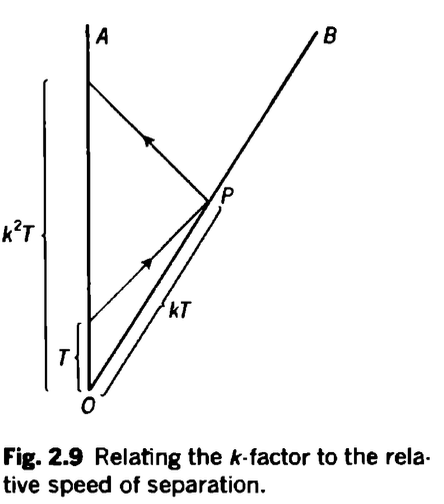
\includegraphics[width=6cm]{Chap1/1-2}\\
	Fig 1-2. assume that $A$ and $B$ synchronize their clocks to zero when they cross at event $O$. After a time $T$, $A$ sends a signal to $B$, which is reflected back at event $P$. From $B$'s pointof view, a light signal is sent to $A$ after a time lapse of $kT$ by $B$'s clock.
	\end{center}
	There are two ways of calculating the $k$-factor, with or without the Lorentz Transform.\\

	\bluebf{Method 1}\\
	
	In this method, we calculate the coordinate of $P$ in $A$'s frame, and apply Lorentz transformation to obtain the time interval measured with $B$'s watch. Let $A_s$ be the event where $A$ sends the signal and $A_r$ be the time $A$ receives the signal from $B$.
	
	We have:
	\begin{align*}
	A_sP:~~&t = x+T\\
	OP:~~	&t = \frac{x}{v}
	\end{align*}
	calculate the coordinate of intersection $P$, we obtain:
	\begin{align*}
	t_P = \frac{1}{1-v}T, x_P = \frac{v}{1-v}T\\
	A_rP:~~ -1(t - t_P) = x - x_P
	\end{align*}
	This gives $k^2T$, or the length of $A_rO$:
	\begin{align*}
	k^2T = \frac{1+v}{1-v}T
	\end{align*}
	We can confirm that the calculation of $k$ is correct by doing the following. With the coordinate of $P$, apply Lorentz transformation:
	\begin{align*}
	t_P' =& \frac{t_P - vx_P}{\sqrt{1 - v^2}} = \sqrt{\frac{1+v}{1-v}}T\\
	x_P' =& t_P' = \frac{x_P - vt_P}{\sqrt{1 - v^2}} = 0	
	\end{align*}
	Therefore, from the perspective of $B$, he did not move in his frame while his time advanced by $\sqrt{\frac{1+v}{1-v}}T$. The calculation in $B$'s frames gives the value of $k$ while the calculation in $A$'s frame gives the value of $k^2$. Since $k_A^2 = k_B^2$, we confirm the calculation result to be correct. \\
	Note, when $B$ is approaching $A$, we can easily obtain the value of $k$ by switching $v$ to $-v$.\\

	\bluebf{Method 2 (book method)}\\
	
	We can simply mark the coordinate the coordinate of P according to $A$'s clock:
	\begin{align*}
	(t_P, x_P)_A = \cb{\frac{1}{2}(k^2+1)T, \frac{1}{2}(k^2-1)T}
	\end{align*}
	we can get velocity form linearity in assumption:
	\begin{align*}
	v = \frac{x}{t} = \sqrt{\frac{1+v}{1-v}}T
	\end{align*}
	Note, we require $k>1$ for separating observers and $k<1$ for approaching observers. This is the commonly known ``Doppler Shift'', while $k>1$ represents a \color{red}redshift\black, and $k<1$ represents a \blue blueshift\black.
	\end{multicols}

	\newpage
	\section{Composition Laws for Velocities}
	Consider the configuration described in Figure 1-3.
	\begin{center}
	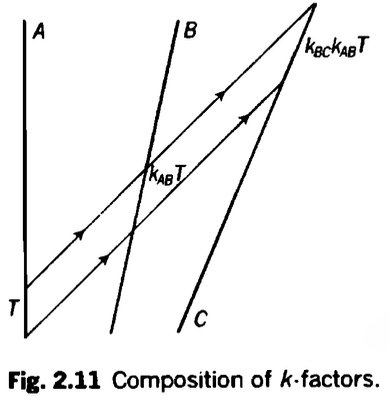
\includegraphics[width=6cm]{Chap1/1-3}\\
	Figure 1-3: In this configuration, there are 3 observers $A,B,C$. $k_{AB}$ denotes the $k$-factor between $A$ and $B$, with $k_{AC}$ and $k_{BC}$ defined similarly. 
	\end{center}
	It follows immediately that	
	\begin{align*}
	k_{AC} = k_{AB}k_{BC}\\
	v_{AC} = \frac{v_{AB}+v_{BC}}{1-v_{AB}v_{BC}}
	\end{align*}
	In the classical limit where $v_{AB}, v_{BC}\ll 1$, we have:
	\begin{align*}
	v_{AC} = v_{AB}+v_{BC}
	\end{align*}
	When either $V_{AB}$ or $V_{BC}$ is the velocity of light, we have:
	\begin{align*}
	v_{AC} = 1
	\end{align*}
	
	
From the composition law, we can show that, fi we add two speeds less than the speed of light, then we again obtain a speed less than the speed of light. This does not mean, as is sometimes stated, that nothing can move faster than the speed of light in special relativity, but rather that the speed of light is a border which can not be crossed or even reached. More precisely, special relativity allows for the existence of three classes of particles: \textbf{subluminal, luminal, and superluminal}.

	\section{Relativity of Simultaneity and Clock Paradox}
	Please refer to \textit{d'Inverno's book section 2.10-2.11} for this. It is straight forward and easy to understand.
	
	The most intriguing concept to me here is the definition of causality and causal contact.
	\begin{center}
	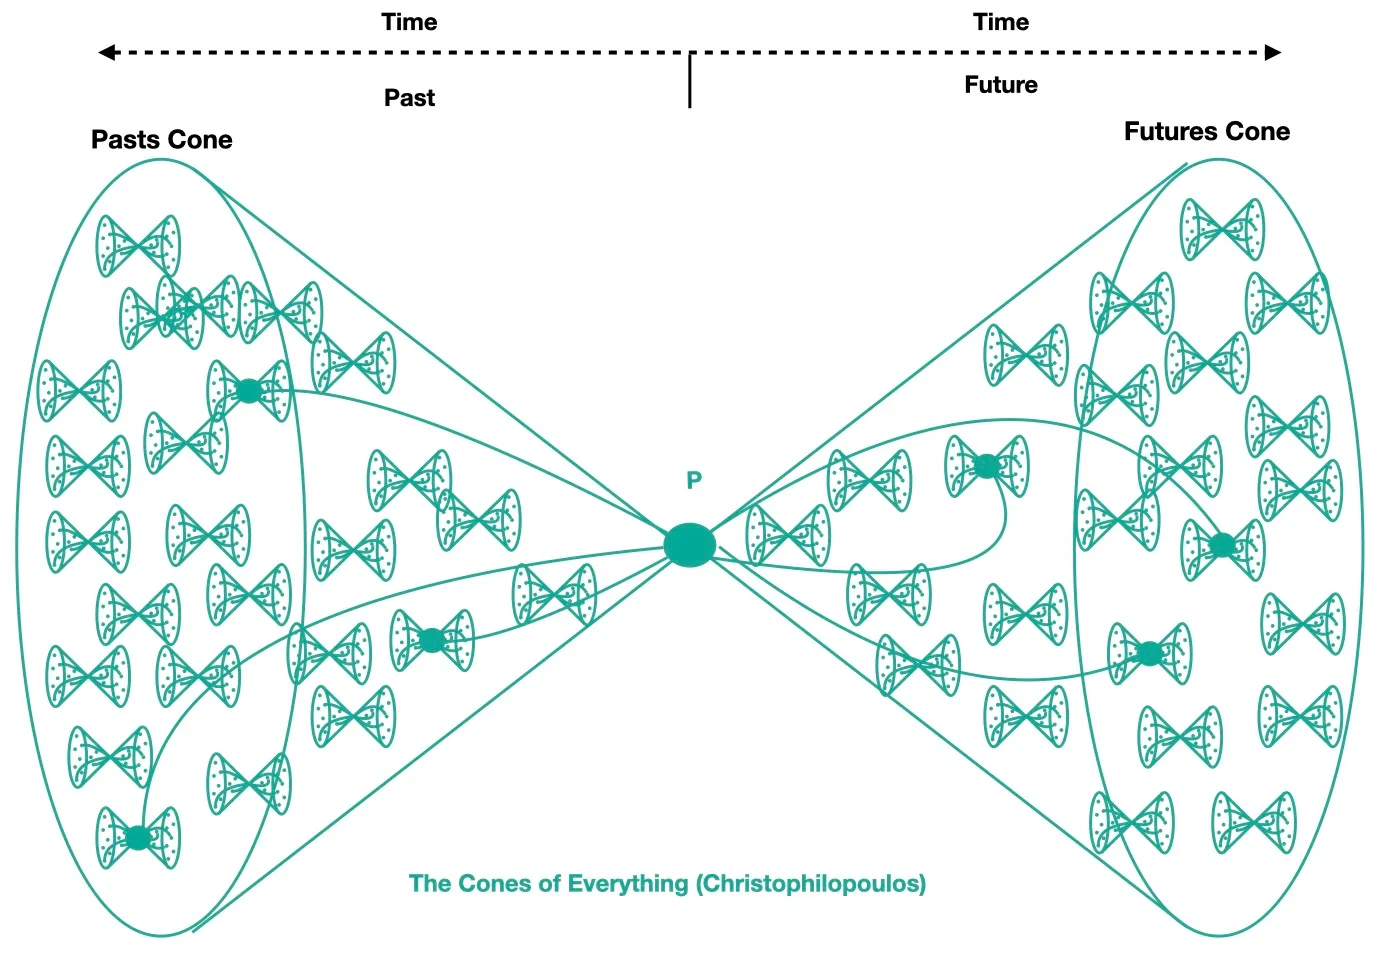
\includegraphics[width=8cm]{Chap1/1-4}
	\end{center}

	\chapter{Key Attributes of Special Relativity}
	
	\section{Standard Derivation of Lorentz Transformations}
	
	\section{}
	
	
\end{document}